\documentclass[a4paper]{article}
\setlength{\parindent}{0pt}

%%%%%%%% CREATE DOCUMENT STRUCTURE %%%%%%%%
%% Language and font encodings
\usepackage[english]{babel}
\usepackage[utf8x]{inputenc}
\usepackage[T1]{fontenc}
%\usepackage{subfig}

%% Sets page size and margins
\usepackage[a4paper,top=3cm,bottom=2cm,left=2cm,right=2cm,marginparwidth=1.75cm]{geometry}

%% Useful packages
\usepackage{framed}
\usepackage{amsmath}
\usepackage{graphicx}
%\usepackage[colorinlistoftodos]{todonotes}
\usepackage[colorlinks=true, allcolors=blue]{hyperref}
\usepackage{caption}
\usepackage{subcaption}
\usepackage{listings}
\usepackage{lstautogobble}
\usepackage{sectsty}
\usepackage{apacite}
\usepackage{float}
\usepackage{titling} 
\usepackage{blindtext}
\usepackage[square,sort,comma,numbers]{natbib}
\usepackage{xcolor}
\definecolor{darkgreen}{rgb}{0.0, 0.4, 0.0}

\definecolor{pblue}{rgb}{0.13,0.13,1}
\definecolor{pgreen}{rgb}{0,0.5,0}
\definecolor{pred}{rgb}{0.9,0,0}
\definecolor{pgrey}{rgb}{0.46,0.45,0.48}

\usepackage{listings}
\lstset{language=Java,
    showspaces=false,
    showtabs=false,
    breaklines=true,
    showstringspaces=false,
    breakatwhitespace=true,
    commentstyle=\color{pgreen},
    keywordstyle=\color{pblue},
    stringstyle=\color{pred},
    basicstyle=\ttfamily,
    colframe=white!75!black,
    moredelim=[is][\textcolor{pgrey}]{\%\%}{\%\%}
}

\usepackage[most]{tcolorbox}

\newtcblisting{shell}{colback=black,colupper=white,colframe=white!75!black,
	listing only,listing options={language=sh}}

% ToDo: List
\usepackage{enumitem,amssymb}
\newlist{todolist}{itemize}{2}
\setlist[todolist]{label=$\square$}

\usepackage{tikz}
\usetikzlibrary{calc,shapes.multipart,chains,arrows, matrix, positioning}

%%%%%%%% DOCUMENT %%%%%%%%
\begin{document}

%%%% Title Page
\begin{titlepage}

\newcommand{\HRule}{\rule{\linewidth}{0.5mm}} 							% horizontal line and its thickness
\center 
 
% University
\textsc{\LARGE University of Illinois @ Urbana-Champaign}\\[1cm]

% Document info
\textsc{\Large CI 487: Data Structures for CS Teachers}\\[0.2cm]
\textsc{\large }\\[1cm] 										% Course Code
\HRule \\[0.8cm]
{ \huge \bfseries Implementation \#2:\\\vspace{0.1cm}Simplified List Interface and ArrayList}\\[0.7cm]								% Assignment
\HRule \\[0.8cm]
%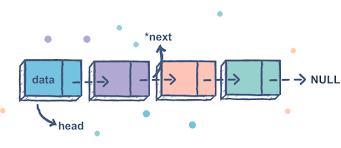
\includegraphics[width=0.6\textwidth]{images/singly-linked-list.png}\\[1cm] 	% University logo
\vfill 
\end{titlepage}

%%\begin{abstract}
%%Your abstract.
%%\end{abstract}

%%%% SECTIONS
%% Section 1
\section*{Objectives and Overview}

Linear data structures are among the most common used in day to day
programming. Throughout this course you have already encountered, utilized, and
analyzed the List interface and it's two most commonly used implementations,
\lstinline|ArrayList| and \lstinline|LinkedList|. In this assignment you will
be building a simplified generic list interface and providing an implementation
that is functionally identical to the real \lstinline|ArrayList| class in Java.
This assignment has the following objectives:
\begin{itemize}
	\item Familiarize you with generics, generic interfaces, and generic classes.
    \item Familiarize you with the underlying implementation of the \lstinline|ArrayList| class.
    \item Understand in which situations to use the \lstinline|ArrayList| implementation rather than \lstinline|LinkedList|.
    \item Provide a basis for comparing this class to the \lstinline|LinkedList| data structure you will implement in the next assignment.
\end{itemize}

\section*{The ArrayList}

\subsection*{Initializing an ArrayList}
At it's heart, an array list is just typical Java array wrapped up into a class
that manages dynamic resizing as it is needed. Recall that to create an empty
list of integers we would use the following line of code where \lstinline|SIZE|
is an integer representing the number of empty slots we want in our array.\\

\begin{lstlisting}[frame=trBL]
Integer[] ints = new Integer[SIZE];
\end{lstlisting}

Let's say \lstinline|SIZE| was defined to be four. After the above operation
was executed we would be left with an array with four blank spaces where we 
could store instances of the \lstinline|Integer| class.\\
\begin{figure}[H]
	\centering
	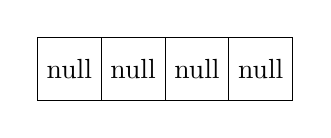
\begin{tikzpicture}
	\matrix (A) [matrix of nodes, nodes={draw, minimum size=8mm},
		column sep=-\pgflinewidth]{
		null & null & null & null \\};
	\end{tikzpicture}
\end{figure}

\subsection*{Adding Elements}
We can then add elements by indexing into various positions in the array and 
putting new integers at each of those positions.\\

\begin{minipage}{0.45\textwidth}
\begin{lstlisting}[frame=trBL]
ints[0] = 2;
ints[1] = 3;
ints[2] = 5;
ints[3] = 7;
\end{lstlisting}
\end{minipage}
\hfill
\begin{minipage}{0.45\textwidth}
\begin{figure}[H]
	\centering
	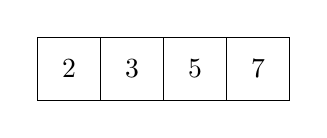
\begin{tikzpicture}
	\matrix (A) [matrix of nodes, nodes={draw, minimum size=8mm},
		column sep=-\pgflinewidth]{
		2 & 3 & 5 & 7 \\};
	\end{tikzpicture}
	\vspace{1.0cm}
\end{figure}
\end{minipage}


However, now we are faced with an issue. Our array is full, what if we want to
add another integer to it? This isn't an \lstinline|ArrayList| so we must manually
``resize'' the array. The purpose of the word ``resize'' is that it is not possible to
just allocate more space at the end of our current array. Rather, we must instantiate 
a new, larger array and copy over all of the elements from the old array to the new 
one. An example of how this might be accomplished manually is shown below along
with a visual of what the \lstinline|moreInts| array would look like
afterwards.\\

\begin{minipage}{0.59\textwidth}
\begin{lstlisting}[frame=trBL, basicstyle=\small]
Integer[] moreInts = new Integer[ints.length + 4];
for(int i = 0; i < ints.length; i++){
	moreInts[i] = ints[i];
}
\end{lstlisting}
\end{minipage}
\hfill
\begin{minipage}{0.39\textwidth}
\begin{figure}[H]
	\centering
	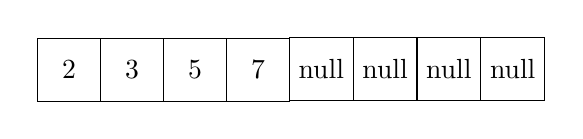
\begin{tikzpicture}
	\matrix (A) [matrix of nodes, nodes={draw, minimum size=8mm},
		column sep=-\pgflinewidth]{
		2 & 3 & 5 & 7 & null & null & null & null \\};
	\end{tikzpicture}
\end{figure}
\vspace{0.3cm}
\end{minipage}

The array's class provides a static method \lstinline|Arrays.copyOf(array, newSize)| 
where \lstinline|array| is the array we want to copy into the larger array and
\lstinline|newSize| is the size of the new array. Using this method we could accomplish the same 
task as above via the following, single line of Java.\\

\begin{lstlisting}[frame=trBL, basicstyle=\small]
Integer[] moreInts = Arrays.copyOf(ints, ints.length + 4);
\end{lstlisting}


This process of dynamically creating new arrays and copy the contents of the
old arrays over to the new one is managed by the \lstinline|ArrayList| class.
This functionality is enabled by the \lstinline|ensureCapcity| method which is
called every time an element is added to an \lstinline|ArrayList|. It checks to
see if there is space exists and, if it doesn't, it performs the process of
allocating a larger array and copying elements to it. 

\textbf{Note:} The provided starter files allow for has a working \lstinline|ensureCapacity| method that uses the 
\lstinline|Arrays.copyOf| method. You will want to use that provided method to complete the rest of the methods
detailed int the assignment. After completing those, come back to the \lstinline|ensureCapacity| method and change
it's implementation to use the manual algorithm detailed above.

\subsection*{Removing Elements}

Now that we know how to filled an array, let's consider the case where we want to remove
elements from the array. Let's consider the following array of primes.  

\begin{minipage}{0.59\textwidth}
\begin{lstlisting}[frame=trBL, basicstyle=\small]
Integer primes = {2, 3, 5, 7, 11, 13, 17, 19};
\end{lstlisting}
\end{minipage}
\hfill
\begin{minipage}{0.39\textwidth}
\begin{figure}[H]
	\centering
	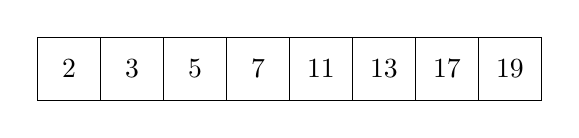
\begin{tikzpicture}
	\matrix (A) [matrix of nodes, nodes={draw, minimum size=8mm},
		column sep=-\pgflinewidth]{
		2 & 3 & 5 & 7 & 11 & 13 & 17 & 19 \\};
	\end{tikzpicture}
\end{figure}
\vspace{0.3cm}
\end{minipage}

If we ``remove'' 11 by simply setting the reference at it's index to
\lstinline|null| we will end up with a hole in the middle of our array. 

\begin{minipage}{0.59\textwidth}
\begin{lstlisting}[frame=trBL, basicstyle=\small]
primes[4] = null;
\end{lstlisting}
\end{minipage}
\hfill
\begin{minipage}{0.39\textwidth}
\begin{figure}[H]
	\centering
	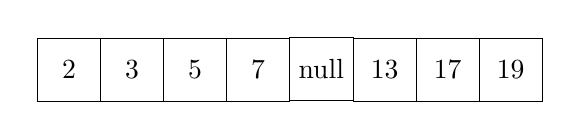
\begin{tikzpicture}
	\matrix (A) [matrix of nodes, nodes={draw, minimum size=8mm},
		column sep=-\pgflinewidth]{
		2 & 3 & 5 & 7 & null & 13 & 17 & 19 \\};
	\end{tikzpicture}
\end{figure}
\vspace{0.3cm}
\end{minipage}

If we continue this process with many add and remove operations we will end up
with a large array with many unfilled holes.

\begin{figure}[H]
	\centering
	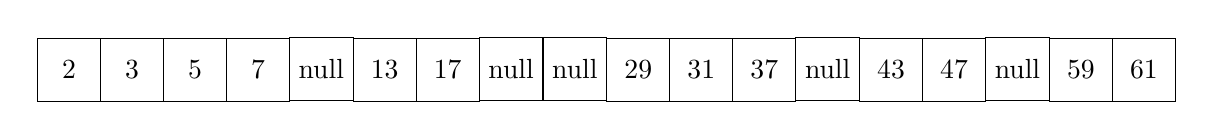
\begin{tikzpicture}
	\matrix (A) [matrix of nodes, nodes={draw, minimum size=8mm},
		column sep=-\pgflinewidth]{
		2 & 3 & 5 & 7 & null & 13 & 17 & null & null & 29 & 31 & 37 & null & 43 & 47 & null & 59 & 61\\};
	\end{tikzpicture}
\end{figure}

So, every time we remove an element we need to ``resize'' the array such that
the ``holes'' caused by setting references to null don't occur. But, as
previously discussed we can't simply expand and shrink arrays. Per the Java docs
the way the \lstinline|ArrayList| class accomplishes this is defined 
by the remove method's documentation:

\begin{quote}
\textit{Remove the element at the specified position in this list. Shifts any
subsequent elements to the left (subtracts one from their indices).}
\end{quote}

 With the documentation in mind, we can see that we don't want to remove the
element by simply setting it equal to null. Rather, we want to shift all of the
elements to the right of that element one position to the left. After engaging
in this process to remove 11 we would be left with the following array.\\

\begin{figure}[H]
\centering
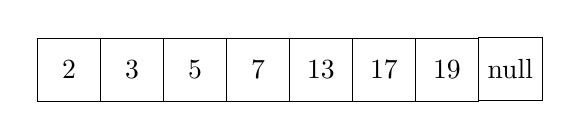
\begin{tikzpicture}
\matrix (A) [matrix of nodes, nodes={draw, minimum size=8mm},
	column sep=-\pgflinewidth]{
	2 & 3 & 5 & 7 & 13 & 17 & 19 & null \\};
\end{tikzpicture}
\end{figure}

This leaves us with two cases that we must consider for the removal of an element:
\begin{itemize}
	\item \textbf{Case 1: } If the element we are attempting to remove is at the end of the array we can simply set it's position in the array to null.
	\item \textbf{Case 2: } If the element we are attempting to remove at the beginning or in the middle then we must shift every element to it's right one position to the left.
\end{itemize}

\section*{Structures and Specifications}

\subsection*{SimpleList Interface}

This will be a generic interface that is very similar to the \lstinline|List<E>|
interface you are already familiar with. The following is a list of method 
prototypes you should have in the interface.

\begin{itemize}
    \item \lstinline|public int indexOf(E e)| 
    \item \lstinline|public void add(E e)| 
    \item \lstinline|public boolean remove(E e)| 
    \item \lstinline|public E get(int i)| 
    \item \lstinline|public boolean contains(E e)| 
    \item \lstinline|public boolean isEmpty()| 
\end{itemize}

The implementation details of these methods will be expanded upon in the
following sections.

\subsection*{SimpleArrayList Class}

\subsubsection*{Attributes}

Your class should have the following attributes
\begin{itemize}
	\item \lstinline|private Object items[]|: This is our list of arbitrary objects. 
	\item \lstinline|private static final int INITIAL_SIZE|: This variable is used by the constructor to create the initial, blank array of Objects. It is \lstinline|final| since it is constant and we don't want it to be changed by the user. It is \lstinline|private| since we don't want it to be accessible outside of the class. Finally, it is \lstinline|static| since we want it accessible anywhere in the class.
	\item \lstinline|private static final int INCREASE_SIZE|: This variable is used by the constructor to create the initial, blank array of Objects. It is \lstinline|final| since it is constant and we don't want it to be changed by the user. It is \lstinline|private| since we don't want it to be accessible outside of the class. Finally, it is \lstinline|static| since we want it accessible anywhere in the class.
	\item \lstinline|private int size|: You might think that we could get length of the \lstinline|items| in order to determine the number of elements. However, recall that we have an array with extra space so the number of filled spaces in the array may not equal the length of the array. As such, we need to keep track of the number of filled spaces in our array through the \lstinline|size| attribute by incrementing it and decrementing when we add and remove elements, respectively.
\end{itemize}

\subsubsection*{Methods}

For this class you will need to provide implementation for each of the methods
defined in the interface as well as an additional method that is specific to
this implementation of our \lstinline|SimpleList| interface.

\textbf{Class Specific Methods:}
\begin{itemize}
    \item \lstinline|private void ensureCapacity(int minCapacity)| This method should see if the array still has space for an additional element. You should call the method with the current size of the array plus one to ensure you have enough room left to include the additional element. This can be achieved by comparing the \lstinline|size| attribute to the total length of the list. If it does not, it should reassign the \lstinline|items| attribute to be a copy of the original array with more space add the end. \\ \textit{For this method we provide an implementation that will allow you to begin working on other aspects of the assignment. After completing ALL other methods, then come back to this method and implement the manual array copy algorithm detailed in the introduction.}
	\item \lstinline|public String toString()|  This method should return a string with each element in the list separated by commas. For the purposes of testing, you are encouraged to override the to string method early on so you can easily output the contents of your list. 
\end{itemize}


\newpage
\textbf{Interface Methods you Must Implement:}
\begin{itemize}
    \item \lstinline|public void add(E e)| Given a new element this method will add that element to the end of the array. However, before adding the element should use the \lstinline|ensureCapacity| method to ensure there is enough space for the new element and resize if needed.
    \item \lstinline|public int indexOf(E e)| This searches the array of elements to see if a given element is present in the list. If it does it should return the index and, if it doesn't, it should return -1. \textit{Hint: You may want to implement this method first as it can be useful when implementing other methods.}
    \item \lstinline|public boolean remove(E e)| The remove method is a bit more complicated. Every time we remove an element we have a hole in the array. As such, every time an element is removed we need to engage in a similar copying process where we allocate a new array and copy over all of the elements from the other array into a new one so all elements are contiguous. If the element that is passed in as a parameter is not found in the list then the internal array should remain the same and \lstinline|false| should be returned. If the element is found the described resizing process should be performed and \lstinline|true| should be returned. \textit{Hint: This may be another good place to use the indexOf function.}
    \item \lstinline|public E get(int i)| This method is the inverse of the\texttt{indexOf} method. Rather than finding the index of an item it \textbf{takes} an index as it's parameter it finds and returns a reference to a given object in the list.If the index is out of bound (i.e., i > size - 1) then we should return \lstinline|null|. 
    \item \lstinline|public boolean contains(E e)| This looks through the internal array and attempts to locate the object that is passed in as a parameter. If that item is found it should return true otherwise it should return false. \textit{Hint: This is another good place to use the indexOf function.}
    \item \lstinline|public boolean isEmpty()| This method returns true if the internal array is empty and false if it is not.
\end{itemize}

\section*{Suggested Testing}

You are provided with a sample file with a main method that creates two
instances of \lstinline|SimpleArrayList|, one that holds instances of
\lstinline|String| and the other contains \lstinline|Integer|. Once you have
implemented all methods you should be able to run that file and get the following
output.


\begin{shell}
.add(E e), toString(), and ensureCapacity() Tests:
1, 2, 3, 4, 5, 6, 7, 8, 9, 10, ... , 100

.indexOf(E e) Tests
The index of 2 is: 1
The index of 3 is: 2
The index of 7 is: 6

.add(E e) and .remove(E e) Tests
hi, hello, hola
hello, hola, ni hao

.get(int i) Method Tests:
We got 'hello' from the list at position 0
We got 'hola' from the list at index 1

.contains(E e) Method Tests:
Is 'hello' in the list? true
Is 'hi' in the list? false

.isEmpty() Method Tests:
Is the empty list empty? true;
\end{shell}
\textit{Note:} The output of the add, toString, and ensureCapacity test should 
output numbers 1-100 in full. This was cut down just for the example output to
avoid a large block of numbers in the pdf.

After that you should further experiment with your methods to ensure that they
work in accordance with the specifications you were given.

\section*{Hints}

\subsection*{String Builder}

Given we are constructing a string in the toString method that has an
arbitrary number of generic elements we will want to use a class called
\lstinline|StringBuilder| that allows us to construct a string iteratively and
then eventually produce a single string at the end.  The following example code
iteratives over a list of arbitrary elements and converts them to a string
separated by arrows and with an arrow pointing to null at the end. You 
will want to modify this code in order to get a set of comma separated 
slements.
\begin{lstlisting}[frame=trBL, basicstyle=\small]
@Override 
public String toString(){
    StringBuilder sb = new StringBuilder();
    for(int i = 0; i < elems.length; i++){
        String elemStr = elems[i].toString(); // Converts the object to a string.
        sb.append(elemStr); // Adds the string to the end of string builder.
        sb.append(" -> ");  // Adds an arrow after the element.
    }
    sb.append(" -> null "); // Adds the final arrow indicating the array is done.
    return sb.toString();
}
\end{lstlisting}

\subsection*{Casting Object to E}

As you might notice we are storing elements in an array of type
\lstinline|Object|, however, our functions are taking and returning
\lstinline|E|. This is because Java does not allow for arrays of type E to be
made so we just instead use \lstinline|Object| to create arrays of abitrary
objects. However, if any of our methods want to return items from the list we 
want those methods return type to be \lstinline|E|. Simply returning an item
from the object array would return a type \lstinline|Object| and thus, and 
error would be produced. To remedy this, we \textit{type cast} the \lstinline|Object|
to be \lstinline|E|, as shown below:
\begin{lstlisting}[frame=trBL, basicstyle=\small]
public E get(int i){
    // ..
    // ..
    return (E) items[i];
}
\end{lstlisting}

\section*{Checklist}
\begin{todolist}
	\item The following methods are defined in the \lstinline|SimpleList| interface:
	\begin{todolist}
		\item \lstinline|public int indexOf(E e)| 
		\item \lstinline|public void add(E e)| 
		\item \lstinline|public boolean remove(E e)| 
		\item \lstinline|public E get(int i)| 
		\item \lstinline|public boolean contains(E e)| 
		\item \lstinline|public boolean isEmpty()| 
	\end{todolist}
	\item The following methods are implemented in the \lstinline|SimpleArrayList| class:
	\begin{todolist}
		\item \lstinline|public String toString()| 
		\item \lstinline|private void ensureCapacity(int minCapacity) //(your own implementation)| 
		\item \lstinline|public int indexOf(E e)| 
		\item \lstinline|public void add(E e)| 
		\item \lstinline|public boolean remove(E e)| 
		\item \lstinline|public E get(int i)| 
		\item \lstinline|public boolean contains(E e)| 
		\item \lstinline|public boolean isEmpty()| 
	\end{todolist}
\end{todolist}


%%\section*{Rubric}


%%\newpage
%%\bibliographystyle{apacite}
%%\bibliography{sample}

\end{document}
